\documentclass[conference]{IEEEtran}
\IEEEoverridecommandlockouts
% The preceding line is only needed to identify funding in the first footnote. If that is unneeded, please comment it out.
\usepackage{cite}
\usepackage{amsmath,amssymb,amsfonts}
\usepackage{algorithmic}
\usepackage{graphicx}
\usepackage{textcomp}
\usepackage{xcolor}
\def\BibTeX{{\rm B\kern-.05em{\sc i\kern-.025em b}\kern-.08em
    T\kern-.1667em\lower.7ex\hbox{E}\kern-.125emX}}
\begin{document}

\title{An Efficient Wait-Free Vector in Rust}

\author{\IEEEauthorblockN{Xavier Banks}
\IEEEauthorblockA{\textit{Grad Student, Dept. Computer Science} \\
\textit{University of Central Florida}\\
Orlando, FL, USA \\
xavier95@knights.ucf.edu}
\and
\IEEEauthorblockN{Dax Borde}
\IEEEauthorblockA{\textit{Grad Student, Dept. Computer Science} \\
\textit{University of Central Florida}\\
Orlando, FL, USA \\
daxborde@knights.ucf.edu}
\and
\IEEEauthorblockN{Camilo Lozano}
\IEEEauthorblockA{\textit{Grad Student, Dept. Computer Science} \\
\textit{University of Central Florida}\\
Orlando, FL, USA \\
clozano@knights.ucf.edu}
\and
\IEEEauthorblockN{Juan Parra}
\IEEEauthorblockA{\textit{Grad Student, Dept. Computer Science} \\
\textit{University of Central Florida}\\
Orlando, FL, USA \\
juan.parra54@knights.ucf.edu}
}

\maketitle

\begin{abstract}

Rust is a new programming language that focuses on high performance, access to low level programming, and painless concurrency. With the introduction of new programming languages, the demand for commonly used data structures written natively is strong. Despite its surge in popularity over the past few years and its focus on concurrency, Rust has a surprisingly small variety of concurrent data structures available. Vectors are used quite frequently in sequential Rust, due to their resizability and constant-time access. However, There are few existing implementations of concurrent vectors in Rust. Thus, we present the first non-blocking and wait-free vector written in Rust, based on Feldman et.al. \cite{main}. The goal of this project is to provide an easy-to-use wait-free vector as a Rust library, and to compare our Rust implementation to other implementations, such as blocking implementations and the original C++ implementation.

\end{abstract}

\begin{IEEEkeywords}
wait-free, rust, efficient, vector, concurrent
\end{IEEEkeywords}

\section{Introduction}

Today, software applications are quite complex and must perform efficiently to keep up with performance demands. It is well known that many applications implement a number of common data structures. These data structures form the foundation of the application, and their performance is closely tied to the efficiency of the application. In this project, we will focus on the vector. A sequential vector is a container that stores a sequence of elements contiguously in memory \cite{main}. This allows for efficient constant-time random access, rather than linear-time. Concurrent vectors use more complex memory models to provide the same functionality for many threads \cite{main}.

Rust has become a popular language for safely building multi-threaded applications, as it was built from the ground up with concurrency in mind \cite{rust}. In contrast to other languages, Rust is very strictly typed, has an excellent compiler, and has excellent memory management \cite{rust}. As a result, Rust will not let you make mistakes that can commonly occur in other languages. For example, segmentation faults are not possible in safe, compilable Rust code.

Another benefit that Rust brings to the table is its memory management; all variables must be declared with a ‘lifetime’ which can either be implied by it’s scope or explicitly in the header of a function. In turn this allows for your code to have efficiently managed memory without really having to worry about how it gets done. In fact one of the drawbacks of both the paper and the C++ implementation is that they do not explain how memory is managed. One of the benchmarks of the C++ code can take up to 10 gigabytes since it is not taking care of freeing memory, presumably because of how complicated it can be to implement. By contrast, our implementation aims to leverage Rust's lifetime and borrowing features to implement a concurrent memory management scheme with significantly less complexity.



\subsection{Problem Statement}

\textbf{The goal for this project is to implement a wait free vector data structure in Rust, and benchmark it an existing C++ implementation.} Specifically we’ll be looking at the paper An Efficient Wait-Free Vector \cite{main}. We will be using the existing C++ implementation of the data structure as our control \cite{cpp}. As far as we know, there is no existing non-blocking vector written in Rust that is available publicly. With this project we seek to be able to implement the key features of the commonly used data structure into a new language. Once we have an equivalent implementation in Rust we will run tests on the two different implementations to see if there is any performance difference between them. We will be looking mainly at speed and memory usage.

\section{Motivation}

In our research for this project it was interesting for us to find that there really were not many similar thread safe shared vectors, much less a wait free one. Not to say it is nonexistent, but for the most part it looks like Rust developers prefer to use some form of channels for sending information between threads. Rust’s package manager is called cargo, and packages are called crates. You can search and find what is available on crates.io . It was a surprise to us when we searched on there that there was no such data structure available. One of our ideas initially was to find a similar one and test our implementation against it. 
What we found when people asked online about how to implement a wait free vector is that most answers were to use already available implementation of channels. It seems that the general consensus is to use those when working in Rust. Unlike thread safe vectors, channels are natively baked into the language, and popular implementations such as Crossbeam.
Another popular available implementation is called ‘lockfree’, it offers a couple of different data structures that are lock free, one of which being a stack, it does not guarantee a wait free property. Although one of the main goals of the structure is to provide a solution to the ABA problem, which also happens to be one of the main goals of the paper our data structure is based on. 
Thus it is our goal to be able to have this data structure published on crates.io and have this implementation be another viable alternative to the more common channels. Additionally once we can then test how much more efficient channels really are in Rust than using a wait free vector (or vice versa).
While it is a good thing as our implementation is more unique this is a challenge because it will be harder to find support when it comes to implementing this solution with Rust’s idiosyncrasies as mentioned above.

\section{Related Work}

Our Rust implementation of a wait-free vector will be primary based on the wait-free vector described by Feldman et. al. in \cite{main}. An open source C++ implementation of the vector described in Feldman et. al. \cite{main} is available at \cite{cpp}. We will use this implementation to evaluate the performance of our Rust implementation.
Feldman et. al. \cite{main} state that theirs is the only wait-free vector in literature at time of publication. The authors \cite{main} also mention that the only other non-blocking vector is \cite{lfvec}, which provides a lock free guarantee, but not a wait free one. Since then, one paper \cite{mrlock} has expanded upon the wait-free vector presented in \cite{main}. However, Deligero et. al. \cite{mrlock} do not attempt to maintain the non-blocking properties of the original vector, and instead use it sequentially in combination with a novel lock. While we will use this paper for reference and additional insights throughout this project, it is not directly useful for solving our proposed problem. 

Thus, the Feldman et. al. \cite{main} vector remains the only wait-free vector in literature.

\cite{main} additionally mentions Intel’s TBB library \cite{tbb}, which provides a concurrent vector. However, the documentation does not specify that this vector is non-blocking, and community discussions heavily indicate that all of the library’s collections are blocking \cite{tbbcomm}. Furthermore, Feldman et. al. \cite{main} indicate that their vector and the lock free vector from Dechev et. al. \cite{lfvec} are the only two non-blocking vectors in existence; the absence of TBB’s vector in this assertion, despite the detailed discussion of TBB in the paper \cite{main}, is conspicuous. Thus, the TBB concurrent vector is most likely a blocking vector, and would not be as useful as the wait-free in applications where progress guarantees are necessary. Nonetheless, we plan to evaluate our Rust implementation by comparing its performance to the TBB vector, along with other blocking vector implementations. 



\section{Implementation}
The following is the breakdown of the tasks required to complete our implementation:

\begin{itemize}

    \item Write the general API for Rust implementation of the vector and its subcomponents
    \item Write the functionality of each method in Rust
    \item Develop a testing environment to extract benchmark performances
    \item Create informal reasoning of corrections regarding the approach
    
    
    \item Reproduce the C++ results for a wait-free vector
    \item Compare benchmarks between the two languages
    \begin{itemize}
        \item Measure performance and memory usage
        \item Test a wide variety of scenarios by running tests with different proportions of each method
    \end{itemize}
    
\end{itemize}

\subsection{Anticipated Challenges}
We anticipate a few challenges with implementing this project: Rust’s strictly typed restrictions, lack of similar data structures in Rust, and the group’s unfamiliarity with the language.

Rust's promise of safe and easy concurrency directly influenced the creation of its strict compiler and type system. Though these features will help us greatly in the long run, we anticipate a few sticking points at the beginning of the project. An example of this strictness is that a basic data structure can’t be simply passed between threads. Rust's concept of ‘ownership’ restricts how a data structure can be passed to it, and once the passing occurs, the data still can't be used outside of the original scope. Simply creating a vector and passing it to as many threads as you want without is not possible. You must wrap the vector in a Mutex and an Arc (atomic reference counter), which will allow you to ‘clone’ the structure. If Arc is used, the structure can then be successfully borrowed, as the compiler detects that Arc can clean up the memory once it leaves the scope of all child threads. 

% Moved from challenges section at the end to here
This is just one example of the increased program complexity required to satisfy the compiler's stringent requirements for memory management. Running into more instances like this is one of our main concerns for this project. Granted, these restrictions are meant to keep programmers safe from segmentation faults and other issues, but they can make implementations of algorithms more complicated. If a part of the wait-free vector algorithm can’t be done in normal Rust, it is possible to override some of its safety features by using a variant called unsafe Rust. Doing so would be a sort of last resort option, once you expose unsafe Rust to your code, you lose many of the guarantees that make Rust special. It allows you to access more lower level controls to the code like you would have in C++, but it is no longer safe.

%Since there are almost no other known implementations of this data structure in Rust, it also needs to be seen if it even is possible

We are expecting to run into many more cases like this throughout the project. Even though the goal is to create a wait-free vector that functions identically to the original implementation, its possible that roadblock may force us to adapt the implementation as we go.



Since our group is using this project as an opportunity to improve our Rust skills, we anticipate running into a few roadblocks along the way. For all of us it is a first time in learning both the concepts of the language, and how it functions differently than others that we know. Rust can be unforgiving, and we may run into big obstacles figuring out how to work around those issues.



\subsection{Plan for Implementation}
To summarize from the above sections, our goal is to implement the wait-free vector from Feldman et. al. \cite{main} in the Rust programming language. In addition to wait-freedom, our implementation will also guarantee linearizability. With this implementation completed, we plan to compare it with a handful of other concurrent vector implementations in both C++ and Rust. We are primarily interested in how our Rust implementation compares to the other implementations with regards to performance, but we are also interested to see if any major changes to the design are necessary.
The goal is to expose the wait-free vector for use in general concurrent programming. Our goal is to allow users to import our crate and use our wait-free vector in their concurrent algorithms without using Rust’s “unsafe” blocks. While our own implementation will most likely require low level pointer manipulation, and thus the use of “unsafe” blocks, we want to avoid exposing this complexity.
Our plan is to support each of the methods that Feldman et. al. support in their original implementation. We first began by creating the structs and traits for the vector itself and the descriptors for each operation. The following are the operations that will be supported followed by a summary and informal reasoning of correctness:
    \begin{itemize}
        \item \verb|pushBack|
        \item \verb|popBack|
        \item \verb|at|
        \item \verb|insertAt|
        \item \verb|eraseAt|
        \item \verb|cwrite|
    \end{itemize}
    
After \verb|pushBack|, \verb|popBack|, and “at” are completed, we can begin the benchmarking process. We will run a large number of each operation in fixed proportions (e.g. 50\% \verb|pushBack|, 30\% \verb|popBack|, and 20\% \verb|at|) and record the average number of operations per second. We run the same performance test on the C++ wait-free vector \cite{cpp, main}, the Intel TBB concurrent vector \cite{tbb}, and a naive coarse grained lock on Rust’s sequential vector. We will compare both the execution time and memory consumption of each algorithm. The memory consumption comparison may be somewhat difficult, as the open source C++ implementation does not implement a memory recycling scheme, and leaks a great deal of memory, but we will do our best to present a worthwhile comparison.

% changed from Approach
\section{Testing}

% Given the difficulty of implementing an efficient wait-free vector for Rust, we divided the tasks up to accomplish this goal. 


\subsection{Reproduce C++}

This section is giving credit to the work of c650 on github for providing a reference point in the C++ implementation \cite{cpp}. Although the entity produced results, we decided it was best to reproduce their results for maximum precision. This was done by extrapolating the code and running several individual tests on components of the wait-free vector, such as \verb|popBack| and \verb|pushBack|. This gave us a starting point to what numbers we should expect after the Rust implementation was completed. While writing the code, we were not sure if the implementation will be better or worse, but as stated before, we were contributing a new data structure to the programming language. This would be provided with performance results and it would be up to the user to determine if the newly created data structure would fit their needs. For example, Figure 1 shows the reproduction of the time it took for popBack and pushBack (insert and delete respectively) operations to take place with 32 threads. 
    
\begin{figure}[h]
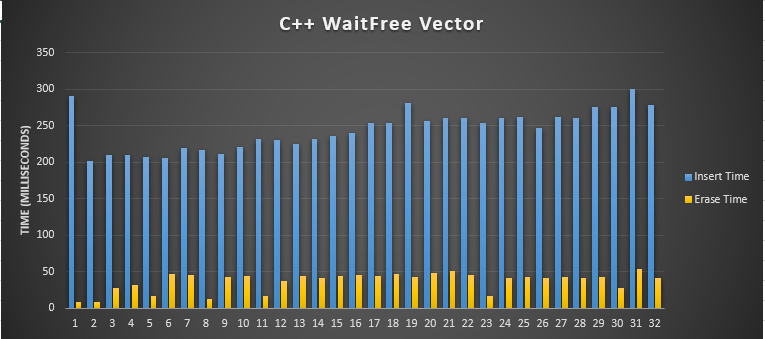
\includegraphics[width=\linewidth]{waitfree_rand_cpp.PNG}
\caption{Results of Waitfree vector in C++}
\end{figure}

% \subsection{API Definitions}

% very broad summary since section {implementation} will talk more about it

\subsection{Testing Environment}

All code was written, compiled, and tested using the standard rust build tools in a Linux environment. This provided a standard across the board to avoid running into OS specific bugs or delays in compilation. 


% \section{Rust Data Structure}

%     \subsection{Runtime/Space Analysis}
    
%     \subsection{Performance}

\section{Evaluation}

    \subsection{Performance Benchmark Results}
    
    \subsection{Limitations}

\subsection{Figures and Tables}

%\section{Challenges}
% Moved a paragraph that was here up to the challenges subsection in the Implementation section above


\bibliographystyle{ieeetr}
\bibliography{references}


\end{document}
